\chapter{Introduction}
\label{ch:introduction}

\newthought{This chapter is for every reader}, whether you have never run a parameter
scan before or you maintain scan infrastructure for a group. It answers three questions
in plain terms: what \Jtwo\ is, how a scan flows through it, and which parts of this
book you personally need. After reading it, you can navigate the rest of the manual by
need instead of by page order.\sidenote{\Jarvis\ stands for \emph{Just a Robust and
Versatile Interface Suite for HEP}. This build documents \Jversion.}

\section{What Jarvis-HEP 2 is}
\label{sec:what-it-does}

\Jtwo\ is a Python framework that runs likelihood-based parameter scans in high-energy
physics.\cite{Guo:2026kfy} You write one \textsc{yaml} file --- the \emph{task card} ---
that says \emph{what} to scan. The runtime handles \emph{how}: it draws parameter
points, runs your physics programs for each point, scores each point with a
log-likelihood, and stores every result.

Think of it as a lab manager for computations.\sidenote{The analogy accompanies the
precise statement; the precise version of every claim in this section follows in
Sections~\ref{sec:mental-model} and~\ref{sec:runtime-picture}.} You hand it a work
order (the task card). It hires a crew (worker processes), gives each member one job at
a time (one parameter point), enforces the safety rules (tool isolation, concurrency
limits), and files every report (databases, logs, summaries) where you can find it
later.

Concretely, the framework solves five problems that otherwise consume your time ---
Table~\ref{tab:at-a-glance} pairs each one with the answer \Jtwo\ gives:

\begin{table}[ht]
  \footnotesize
  \begingroup
  \setlength{\tabcolsep}{0pt}
  \begin{tabular}{@{}p{0.34\linewidth}p{0.66\linewidth}@{}}
    \toprule
    \textbf{Problem} & \textbf{Jarvis-HEP 2 answer} \\
    \midrule
    Running external programs (\textsc{spheno}, \textsc{madgraph}, \ldots) for
      thousands of points & An orchestrated workflow: input files written, commands
      run, outputs parsed --- per point, automatically
      (Part~\ref{part:backends}) \\
    Choosing \emph{which} points to compute & Five sampling methods, from uniform
      random to an adaptive contour tracer (Part~\ref{part:samplers}) \\
    Using a whole machine, not one core & A distributed runtime that scales to
      hundreds of parallel worker processes (Section~\ref{sec:runtime-picture}) \\
    Keeping results usable & \textsc{hdf5} + \textsc{csv} tables with a stable layout
      (Chapter~\ref{ch:outputs}) \\
    Surviving crashes and interruptions & Checkpoints every 30 seconds; resume with no
      lost and no duplicated points (Chapter~\ref{ch:checkpoint}) \\
    \bottomrule
  \end{tabular}
  \endgroup
  \caption{What the framework does for you, at a glance.}
  \label{tab:at-a-glance}
\end{table}

\begin{jnote}
Requirements in one line: \textbf{Python 3.10+}, macOS or Linux, and a local
\textbf{Redis} service (Chapter~\ref{ch:installation} installs both in minutes).
\Jtwo\ is released under the \textsc{mit} License.
\end{jnote}

\section{How one point is processed}
\label{sec:mental-model}

Every scan repeats the same three-step loop, once per parameter point:

\begin{enumerate}
  \item \textbf{Draw a point.} A \emph{sampler} --- the algorithm you pick under
        \yamlkey{Sampling} --- proposes one set of parameter values.
  \item \textbf{Turn the point into observables.} Your workflow runs: external
        \emph{calculators} (file-based physics programs)\sidenote{Whatever the program
        actually is --- a spectrum generator, a dark-matter code, a recasting tool, your
        own script --- \Jtwo\ treats it as a \emph{black box}: write one input file, run
        it, read one output file back. It never parses or understands the program
        itself. Chapter~\ref{ch:quickstart} works this through end to end with a
        four-line example; Chapter~\ref{ch:calculators} is the full reference.} and
        in-process \emph{operas} (Python functions) compute named results such as
        masses or cross sections.
  \item \textbf{Score the point.} Expressions under \yamlkey{Sampling.LogLikelihood}
        combine the observables into a \code{LogL} value.
\end{enumerate}

\begin{marginfigure}
\centering
\smallcaps{point}\\[2pt]
$\big\downarrow$ \emph{sampler}\\[2pt]
\smallcaps{workflow}\\[2pt]
$\big\downarrow$ \emph{calculators / operas}\\[2pt]
\smallcaps{observables}\\[2pt]
$\big\downarrow$ \emph{LogLikelihood}\\[2pt]
\smallcaps{score}
\caption[The per-point loop.]{The per-point loop. Every task card fills in these three
arrows --- notice how each maps to one card block.}
\label{fig:per-point-loop}
\end{marginfigure}

Memorise Figure~\ref{fig:per-point-loop}. Every block in the task card configures one
of its arrows, and Part~\ref{part:task-card} walks the card block by block in exactly
this order.

\section{How a whole scan runs}
\label{sec:runtime-picture}

\begin{figure}[ht]
\centering
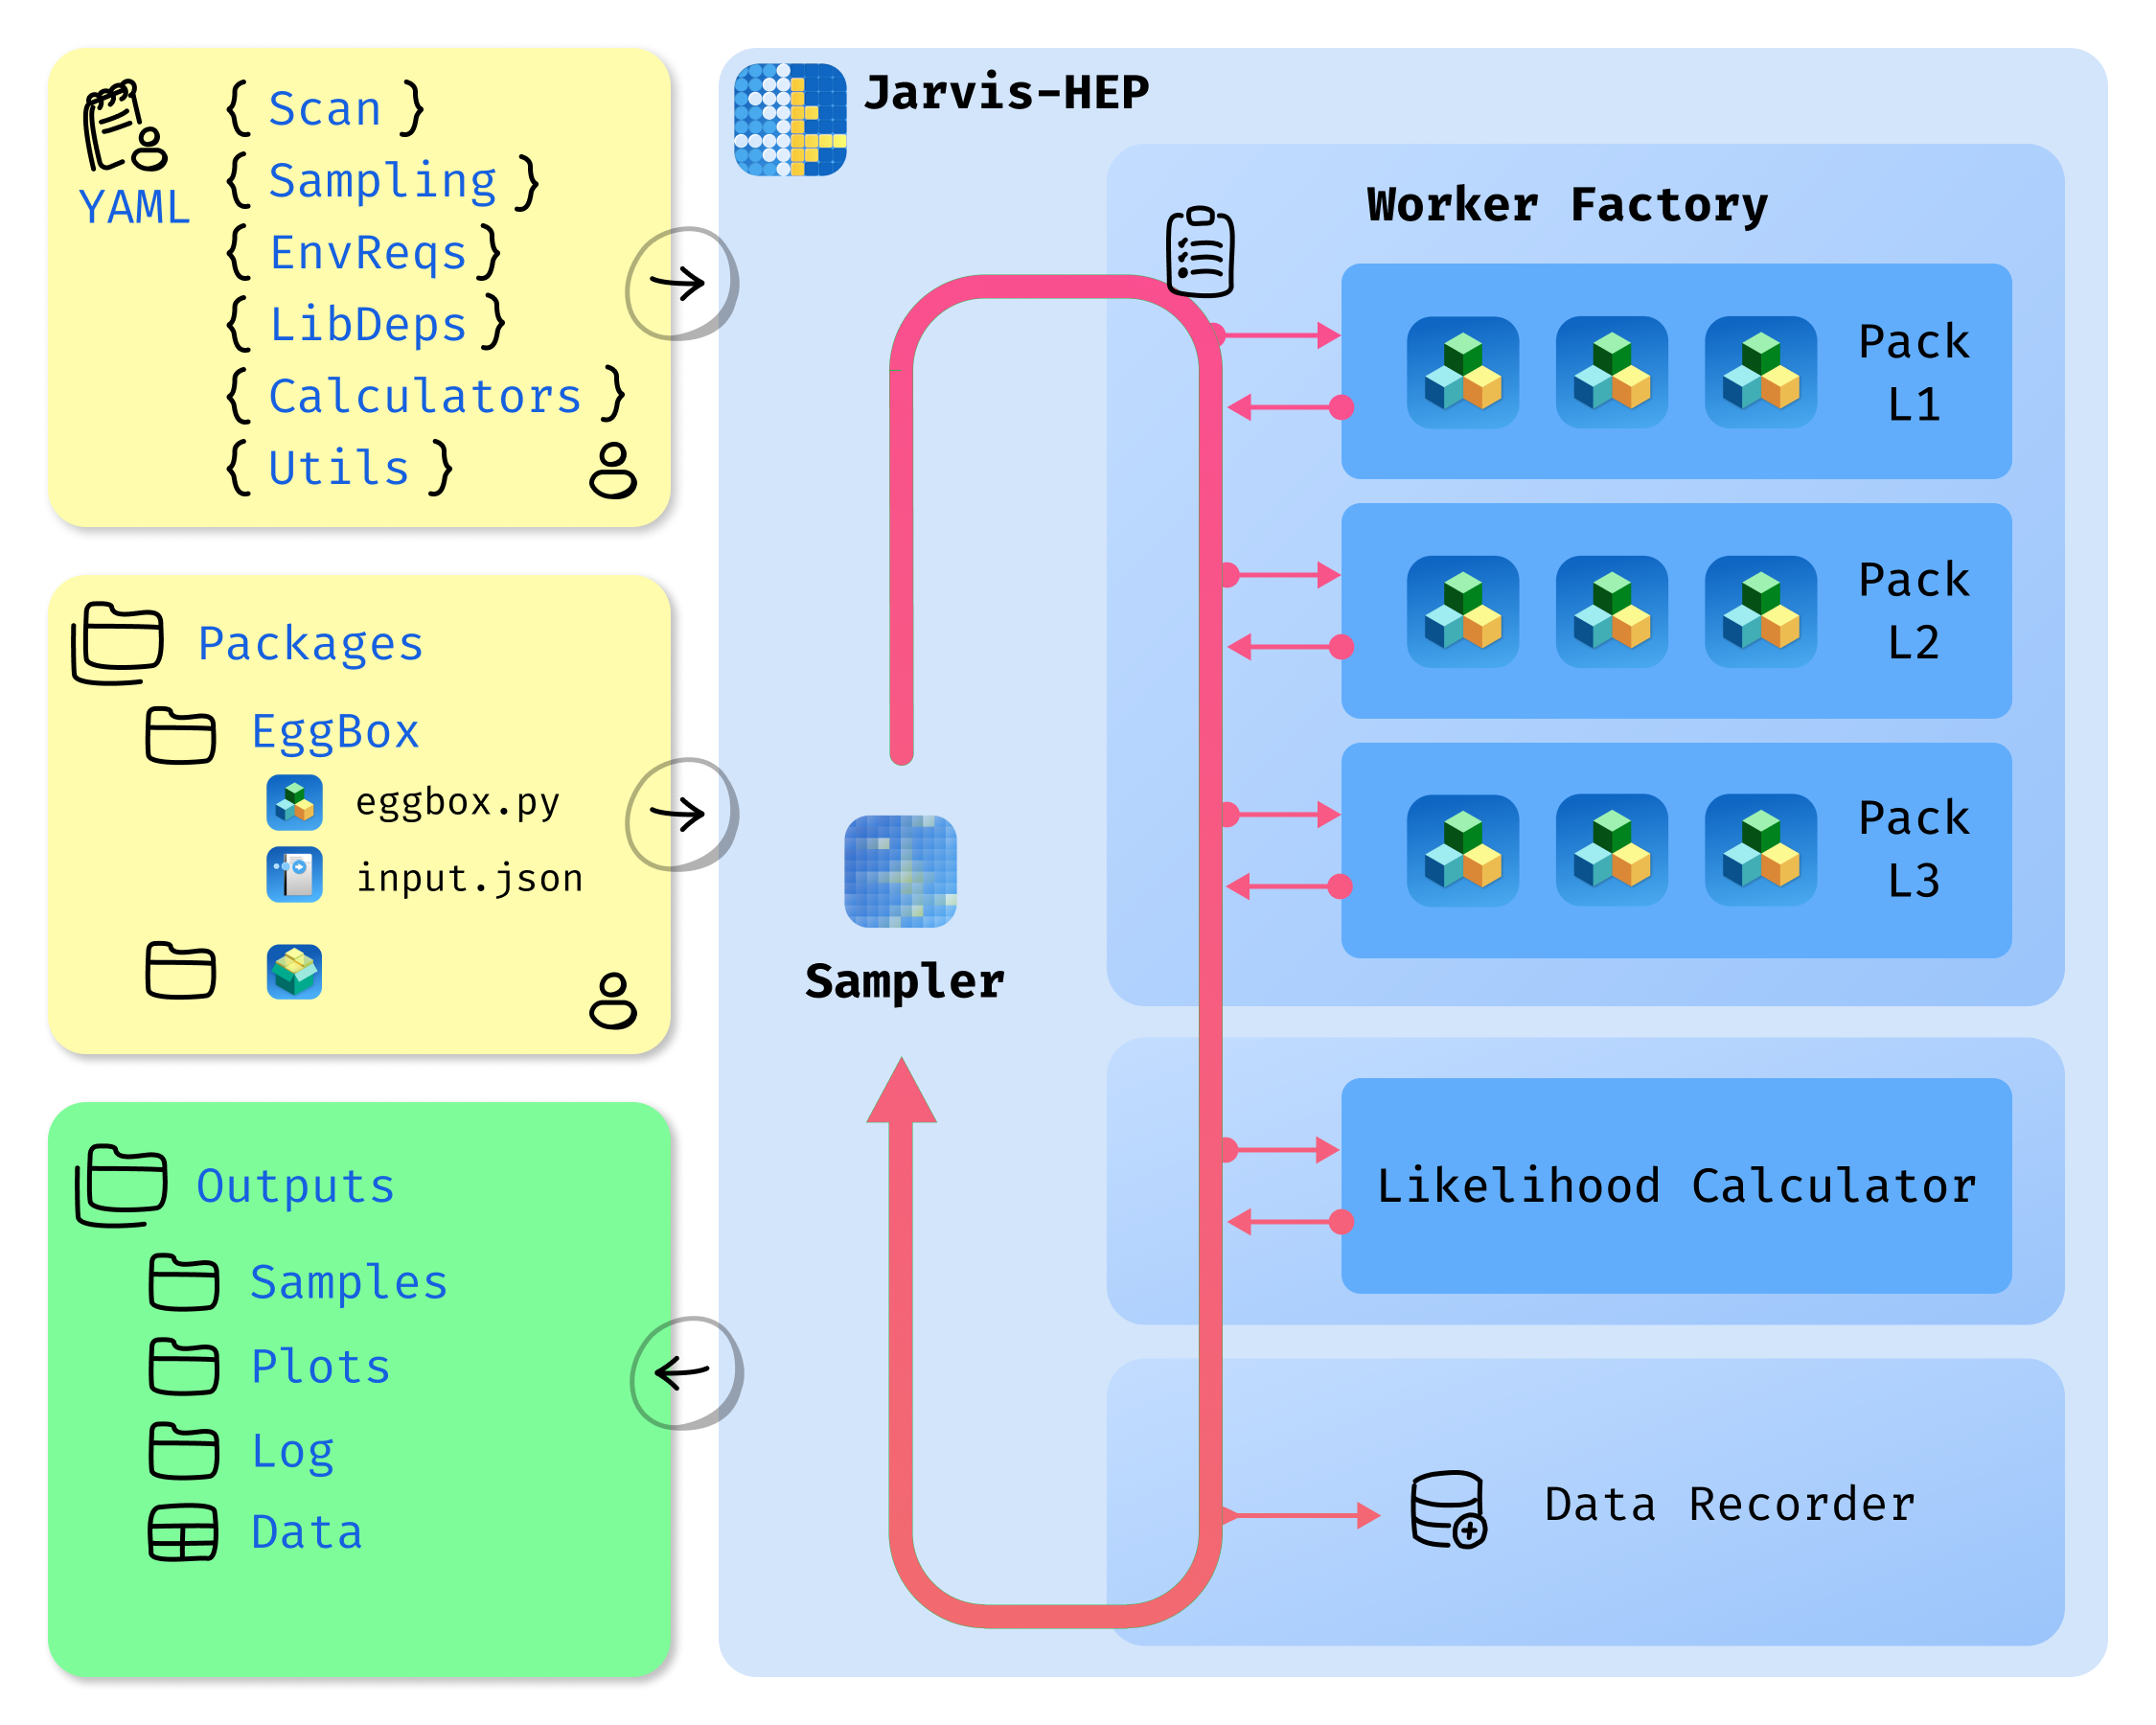
\includegraphics[width=0.85\linewidth]{figures/concept-flow.png}
\caption[The Jarvis-HEP concept, at a glance.]{The \Jarvis\ workflow concept, as
published in the original paper.\cite{Guo:2026kfy} Left to right: you provide the
\textsc{yaml} task card and any external \emph{packages} (yellow); the framework runs
the scan and hands back \textsc{hdf5}/\textsc{csv} tables, plots, and logs (green). The
blue panel's vocabulary is version~1's --- \emph{Worker Factory}, per-package
\emph{module pools} in layers \code{L1}--\code{L3}, a \emph{Data Recorder} --- \Jtwo\
kept the same shape under new names: \code{TaskFactory} (Worker lifecycle only,
Section~\ref{sec:runtime-picture}), per-Sample \emph{layers}
(Chapter~\ref{ch:workflow-model}), and the \emph{Archiver}. The sixth \textsc{yaml}
block shown, \code{Utils}, is now covered by \yamlkey{Operas}
(Section~\ref{sec:card-shape}).}
\label{fig:concept-flow}
\end{figure}

A running scan is a small team of cooperating processes. One parameter point, together
with its files and logs, is called a \emph{Sample} --- the unit of work everything
below passes around.

\begin{quote}
\sffamily\footnotesize
Sampler $\rightarrow$ Redis task queue $\rightarrow$ $N\times$ Workers $\rightarrow$
Archiver $\rightarrow$ \textsc{hdf5}/\textsc{csv}
\end{quote}

\begin{enumerate}
  \item The \textbf{Sampler} (in the control process) proposes points and pushes small
        task descriptions onto a queue.
  \item \textbf{Redis}, a lightweight data service, holds that queue --- plus all
        counters and locks. It is the only thing the processes share.
  \item Each \textbf{Worker} is a long-lived process. It pulls one Sample at a time,
        runs the three-step loop of Section~\ref{sec:mental-model}, and reports the
        result. Independent calculators within one Sample run concurrently.
  \item The \textbf{Archiver} writes finished Samples to the database in batches, off
        the Workers' critical path.
\end{enumerate}

Three design decisions follow from this picture, and they explain most defaults you
will meet later:

\begin{itemize}
  \item \textbf{One runtime path.} There is no single-process or thread mode. Every
        scan --- including a 20-point test --- uses Redis plus spawned Workers, so
        behavior never changes between "testing" and "production".
  \item \textbf{Built for slow calculators.} The target workload is external programs
        that take seconds to minutes per point. The framework's job is to keep many of
        them busy and to persist results cheaply --- not to shave microseconds.
  \item \textbf{Initialise once, reuse always.} Whatever can be loaded once per Worker
        is: program templates, environments, compiled expressions. A Worker's
        thousandth Sample pays none of its first Sample's setup.
\end{itemize}

\begin{jnote}
Failure is a normal outcome, not an emergency. A point whose calculator crashes is
recorded as \emph{failed}, keeps its log for inspection, and the scan continues. One
bad point never aborts a night's work.
\end{jnote}

\Jtwo's concurrency does not stop at ``run many points at once.'' Figure~\ref{fig:concept-flow}
draws two independent axes of it together.

The first axis is ordinary: across Samples, every idle Worker just pulls the next point
off the same Redis queue. Most comparable scan frameworks, such as
\code{EasyScan\_HEP}\cite{Shang:2023gfy} and \code{BSMArt}\cite{Goodsell:2023iac}, are
built around exactly this axis --- they connect a per-point workflow to a sampler and
parallelise by running many points at once.

\Jtwo\ adds a second axis, \emph{inside} each Sample: a point's own calculators run
concurrently with each other too, whenever their declared dependencies allow it --- the
figure's layered blue panel. Concretely, \Jtwo\ turns \yamlkey{required\_modules} into a
dependency graph and runs every calculator that graph allows into the same \emph{layer}
at once (Chapter~\ref{ch:workflow-model}), rather than running one point's calculators
one after another just because they share a point. One point's own wall-clock time
shrinks along with the whole scan's throughput.



\section{What a finished run gives you}
\label{sec:what-you-produce}

Every run writes a predictable, self-contained tree under your project
(Chapter~\ref{ch:outputs} covers each file):

\begin{itemize}
  \item \file{outputs/<scan>/DATABASE/} --- \file{samples.hdf5} and a full
        \file{samples.csv}: one row of observables per point.
  \item \file{outputs/<scan>/SAMPLE/} --- per-point artifacts you chose to keep, in
        bounded, numbered folders.
  \item \file{outputs/<scan>/run\_summary.*} --- counters and throughput, in
        \textsc{json}, \textsc{csv}, and plain text.
  \item \file{logs/} --- one high-level log per process, plus one detailed log per
        point.
\end{itemize}

\section{The package family}
\label{sec:ecosystem}

\Jtwo\ delegates specialised jobs to sibling packages. Two install automatically; one
is optional. Upgrading a sibling adds features without a runtime release.
Table~\ref{tab:ecosystem} names all three and what each is responsible for.

\begin{table}[ht]
  \footnotesize
  \begingroup
  \setlength{\tabcolsep}{0pt}
  \begin{tabular}{@{}p{0.255\linewidth}p{0.213\linewidth}p{0.532\linewidth}@{}}
    \toprule
    \textbf{Package} & \textbf{Install} & \textbf{Role} \\
    \midrule
    \Jtwo   & this manual & sampling, distribution, orchestration, persistence \\
    \Portal & automatic   & file formats for calculator I/O --- \textsc{json},
              \textsc{csv}, \textsc{slha}, \ldots\ (Section~\ref{sec:format-catalog}) \\
    \Operas & automatic   & registry of reusable Python operators and expression
              functions (Chapter~\ref{ch:jarvis-operas}) \\
    \JPlot  & optional \code{[plot]} extra & \textsc{yaml}-driven figures from scan
              outputs (Chapter~\ref{ch:jarvisplot}) \\
    \bottomrule
  \end{tabular}
  \endgroup
  \caption{The \Jarvis\ package family.}
  \label{tab:ecosystem}
\end{table}

\Jtwo\ ships as its own package (\code{jarvishep2}) with its own command
(\cli{Jarvis}). It installs side by side with a version~1 installation without
conflict, and this book assumes no knowledge of that older line --- every concept used
here is defined here.

\section{Your reading path}
\label{sec:next}

Pick the row of Table~\ref{tab:reading-paths} that describes you:

\begin{table}[ht]
  \footnotesize
  \begingroup
  \setlength{\tabcolsep}{0pt}
  \begin{tabular}{@{}p{0.34\linewidth}p{0.66\linewidth}@{}}
    \toprule
    \textbf{You are\ldots} & \textbf{Read\ldots} \\
    \midrule
    new --- nothing installed yet & Chapters~\ref{ch:installation}
      and~\ref{ch:quickstart}, in order; then Chapter~\ref{ch:core-concepts} \\
    writing your first real card & Chapter~\ref{ch:core-concepts}, then
      Part~\ref{part:task-card} block by block \\
    wiring in an external program & Chapters~\ref{ch:workflow-model} and~\ref{ch:calculators},
      with Chapter~\ref{ch:command-system} open \\
    choosing a sampling strategy & Chapter~\ref{ch:choosing-sampler}, then that
      method's chapter \\
    operating and debugging scans & Part~\ref{part:running}, plus
      Appendix~\ref{app:troubleshooting} \\
    tuning or extending the system & Part~\ref{part:advanced} \\
    just looking something up & Chapter~\ref{ch:cli} (commands) or
      Section~\ref{sec:part2-map} (which chapter owns a key) \\
    \bottomrule
  \end{tabular}
  \endgroup
  \caption{Reading paths by need.}
  \label{tab:reading-paths}
\end{table}

\begin{jtip}
If you remember two things from this chapter, keep the two pictures: the per-point
loop (Figure~\ref{fig:per-point-loop}) and the Sampler $\rightarrow$ Redis
$\rightarrow$ Workers $\rightarrow$ Archiver pipeline
(Section~\ref{sec:runtime-picture}). Every feature in this book hangs off one of the
two.
\end{jtip}
